\documentclass[12pt]{article}
\usepackage{mathtools}
\addtolength{\textheight}{.5in}
\addtolength{\textwidth}{1in}
\addtolength{\topmargin}{-.25in}
\addtolength{\evensidemargin}{-.5in}
\addtolength{\oddsidemargin}{-.5in}
\usepackage{placeins}
\begin{document}

\section{Scale factor as a function of time}
From the Friedmann Equation we have
$$ (\frac{\dot{a}}{a})^{2} = \frac{8\pi G}{3}[\rho_{m} + \rho_k + \rho_r + \rho_{\Lambda}] $$
$$ \frac{\dot{a}}{a} = (\frac{8\pi G}{3})^{1/2}[\rho_{m} + \rho_k + \rho_r + \rho_{\Lambda}]^{1/2}$$

In homework 1 we worked out that the ith species $\rho_i = \rho_{0 i}a^{\alpha}$ for alpha equal to -4, -3, -2, 0, 2 for relativistic, non-relativistic, lambda, and curvature matter respectively. If we take a flat model universes with only relativistic or non-relativistic matter, we can solve the Friedmann Equation in the following way

$$ \frac{\dot{a}}{a} = (\frac{8\pi G}{3})^{1/2}[\rho_{i}(a)]^{1/2} $$
$$ \frac{\dot{a}}{a} = (\frac{8\pi G \rho_{0 i}}{3})^{1/2}a^{\alpha/2} $$
$$ \frac{da}{dt} \frac{1}{a} = (\frac{8\pi G \rho_{0 i}}{3})^{1/2}a^{\alpha/2} $$
$$ da \frac{1}{a} a^{-\alpha/2}= (\frac{8\pi G \rho_{0 i}}{3})^{1/2} dt $$
$$ da  a^{-\alpha/2 -1}= (\frac{8\pi G \rho_{0 i}}{3})^{1/2} dt $$
$$ a^{-\alpha/2} \frac{1}{-\alpha/2} = (\frac{8\pi G \rho_{0 i}}{3})^{1/2} t + C$$
$$ a(t)  = [\frac{-t\alpha}{2} (\frac{8\pi G \rho_{0 i}}{3})^{1/2}  -C \alpha/2]^{-2/\alpha} $$

The initial condition $a(0) = 0$ requires that the integration constant is zero. The other condition $a_0 = a(t_0)$ can be used to show
$$a_0  = [\frac{-t_0 \alpha}{2} (\frac{8\pi G \rho_{0 i}}{3})^{1/2}]^{-2/\alpha}$$
$$a_{0}^{-\alpha/2} \frac{2}{-t_0 \alpha} = (\frac{8\pi G \rho_{0 i}}{3})^{1/2}$$

Finally, for a relativistic matter only universe we have alpha=-4, which gives us the solution
$$a_{r}(t)  = (\frac{t}{t_0 })^{1/2} a_{0}$$

For non-relativistic matter only universe we have alpha = -3, which gives us the solution
$$ a_{m}(t)  = (\frac{t}{t_0})^{2/3} a_0$$

The Friedmann equation for a $\rho_{\Lambda}$ universe will lead us to

$$ da \frac{1}{a} = (\frac{8\pi G \rho_{\Lambda}}{3})^{1/2} dt $$
$$ \ln a =  (\frac{8\pi G \rho_{\Lambda}}{3})^{1/2} t + C$$
$$a(t) = \exp[(\frac{8\pi G \rho_{\Lambda}}{3})^{1/2} t]  C'$$

Enforcing the condition $a(t_0) = a_0$ gives us 
$$a_0 = \exp[(\frac{8\pi G \rho_{\Lambda}}{3})^{1/2} t_0]  C'$$
$$\frac{\ln a_0/C'}{t_0} = (\frac{8\pi G \rho_{\Lambda}}{3})^{1/2} $$

$$a(t) = \exp[\ln (a_0/C') t/ t_{0}]  C'$$

\section{Equation of state}
If we parameterize the equation of state for dark energy with $w(a) = w_0 + w_{a}(1 - a)$, the dark energy density becomes

$$ \omega_{Q} = \omega_{Q 0}a^{-3(1 + w(a))}$$
$$ \omega_{Q} = \omega_{Q 0}a^{-3(1 + w_0 + w_{a}(1 - a))}$$

\section{Homogenius Scalar Field}
\subsection{Equation of motion}
The equation of motion is $\ddot{\phi} + 3H\dot{\phi} + V'(\phi) = 0$. We can rewrite H by using the Friedmann equation $\frac{8 \pi G}{3} (\rho_m + \rho_{\phi}) = H^2$.  Additionally, our potential $V(\phi) = V_{0}e^{-\lambda \phi}$, which we use to evaluate $V'(\phi) = \frac{\partial V}{\partial \phi} = -\lambda V_{0}e^{-\lambda \phi} = -\lambda V(\phi)$. Throwing all of this together, the equation of motion becomes

$$\ddot{\phi} + 3\Big[ \frac{8 \pi G}{3} \rho_{tot} \Big]^{1/2}\dot{\phi} - \lambda V(\phi) = 0$$

Now from the stress energy tensor, we have $\rho_{\phi} = \dot{\phi}^2 + V(\phi)$. If we require $V(\phi) = \frac{1}{2} \rho_{\phi}$, we can use the stress energy tensor relation to get the relationship $\rho_{\phi} = \dot{\phi}^2$. Now the equation of motion is 

$$\ddot{\phi} + 3\Big[ \frac{8 \pi G}{3} \rho_{tot} \rho_{\phi} \Big]^{1/2} - \frac{\lambda}{2} \rho_{\phi} = 0$$

Keeping an eye towards what is to come in the next question, we divide through by $\rho_{\phi} $ so that the term $\rho_{tot}/ \rho_{\phi} $ crops up. We then use $\rho_{\phi} = \dot{\phi}^2$ once more. Now we assert if the matter density is always a fixed fraction of the scalar field density, the fraction $\rho_{tot}/ \rho_{\phi}$ is fixed for all times. Now we have an equation in terms of $\phi$, time, and constants only.

 $$\ddot{\phi} \frac{1}{\dot{\phi}^2} + 3\Big[ \frac{8 \pi G}{3} \frac{\rho_{tot}}{ \rho_{\phi}} \Big]^{1/2} - \frac{\lambda}{2} = 0$$
 
 For the sake of readabiltiy, let us define $3\Big[ \frac{8 \pi G}{3} \frac{\rho_{tot}}{ \rho_{\phi}} \Big]^{1/2} - \frac{\lambda}{2} = \kappa $. To tackle the differential equation, let us re-write the equation of motion as a first order equation. We define $f = \dot{\phi}, \dot{f} = \ddot{\phi}$. Now we slide things around, separate variables, and integrate. 
 
 $$\frac{d f}{d t} = -\kappa f^2 $$
 $$ \frac{df}{f^2} = -\kappa dt$$
 $$ \frac{1}{f} = \kappa t + C_1 $$
 $$ f = \frac{1}{\kappa t - C_1} $$
 $$ d\phi = \frac{1}{\kappa t - C_1} dt$$
 $$ \phi(t) = \frac{1}{\kappa} \ln(\kappa t - C_1) + C_2 $$
 
Where $C_1, C_2$ are integration constants. Now we have shown a solution exists for the EOM given the assumptions in the problem.

\subsection{$\rho_{\phi}/\rho_{tot}$ in terms of $\lambda$}

We can eliminate the integration constants from our solution for the scalar field by using the relationship $\rho_{\phi} = 2V(\phi) = \dot{\phi}^2$

$$ \frac{d\phi}{dt} = \sqrt{2V_0}e^{-\lambda \phi/2} $$
$$ d\phi e^{\lambda \phi/2}= \sqrt{2V_0} dt$$
$$  \frac{2}{\lambda} e^{\lambda \phi/2}= \sqrt{2V_0} t + C_3$$
$$ e^{\lambda \phi/2}= \lambda \sqrt{V_{0}/2} t + \frac{\lambda}{2}C_3$$
$$ \phi(t)= \frac{2}{\lambda} \ln  \Big(\lambda \sqrt{V_{0}/2} t + \frac{\lambda}{2}C_3 \Big)$$

Now at time = 0 and $\phi(0) = \phi_0$ we have
$$ e^{\lambda \phi_{0}/2} =  \frac{\lambda}{2}C_3$$
$$ \frac{2}{\lambda} e^{\lambda \phi_{0}/2} = C_3$$
$$ \phi(t)= \frac{2}{\lambda} \ln  \Big(\lambda \sqrt{V_{0}/2} t + e^{\lambda \phi_{0}/2} \Big)$$

Comparing terms of this solution to our previous solution of $\phi$ which solved the EOM, we must conclude $\frac{2}{\lambda} = \frac{1}{\kappa}$

$$ \frac{\lambda}{2}  = 3\Big[ \frac{8 \pi G}{3} \frac{\rho_{tot}}{ \rho_{\phi}} \Big]^{1/2} - \frac{\lambda}{2} $$
$$ \lambda^2 = 24 \pi G \frac{\rho_{tot}}{ \rho_{\phi}}$$
$$ \frac{24\pi G}{\lambda ^2}  = \frac{\rho_{\phi}}{ \rho_{tot}}$$

\subsection{limits on $\lambda$}

In order to keep the appropriate form of the potential, $\lambda$ must be non negative and non zero. Additionally, if this model universe contains matter in addition to the scalar field, the ratio  $\frac{\rho_{\phi}}{ \rho_{tot}} < 1$. All this together tells us that

$$  \lambda > \sqrt{24 \pi G} $$ 

\section{Numerical solutions}
\subsection{Exponential prefactor Potential}
Please see Figure 1
\begin{figure}
\centering
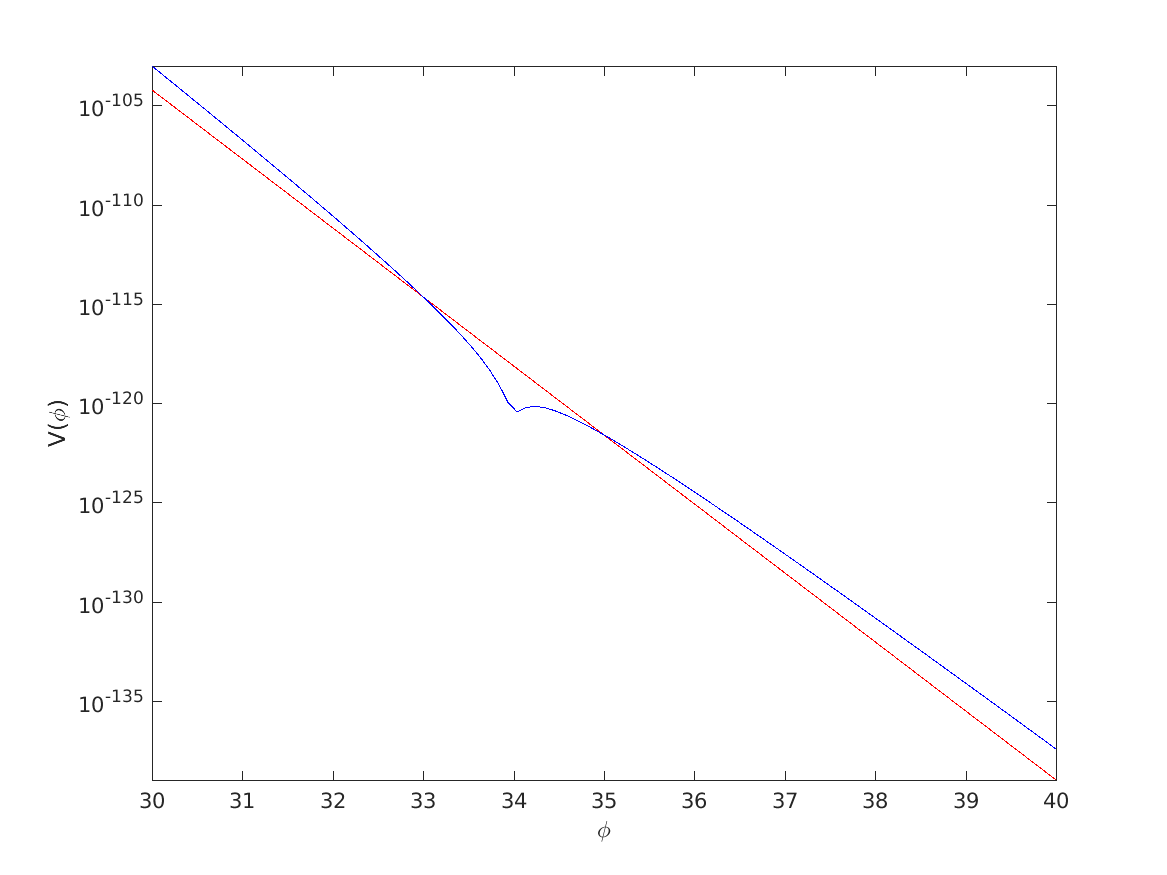
\includegraphics[width=5in]{potential.png}
\caption{the exponential potential and exponential prefactor as a function of $\phi$. The parameters are set to $\lambda = 8$, $\beta$ = 34, $V_0 = 1$, $\delta = 0.005$, $\chi = 1$, $\phi_0 = \beta 1\mathrm{e}-3$}
\end{figure}

\subsection{Approximate the analytic solution}
First we examine the exponential prefactor potential.

$$ V(\phi) = V_{0}(\chi(\phi - \beta)^{2} + \delta)e^{-\lambda \phi}$$

For $\phi \ll \beta$ we can expand  $\phi / \beta$ to first order.

$$ V(\phi) = V_{0}(\chi \phi^2 + \chi \beta^2 - 2\chi\phi\beta) + \delta)e^{-\lambda \phi}$$
$$ V(\phi) = V_{0}\chi\beta^{2}((\frac{\phi}{\beta})^2 + 1 - 2\chi\frac{\phi}{\beta} + \frac{\delta}{\chi\beta^2})e^{-\lambda \phi}$$

Now since $\phi \ll \beta$, $\delta \ll \beta^2$

$$ V(\phi) \approx V_{0}\chi\beta^{2}(1 - 2\chi\frac{\phi}{\beta})e^{-\lambda \phi}$$
$$ V(\phi) \approx V_{0}\chi\beta^{2}e^{-\lambda \phi} - 2V_{0}\chi\phi\beta e^{-\lambda \phi}$$

By inspection, in this limit the potential looks like the exponential potential from question 3 with a first order correction term subtracted off. Only now we have to substitute $V_{0} \to V_{0}\chi\beta^2$. 

Now we will compare the numerical solution of $\phi(t)$ to the analytical solution. When calculating The analytical solution, we will use $V(\phi) \approx V_{0}\chi\beta^{2}e^{-\lambda \phi}$.

\begin{figure}
\centering
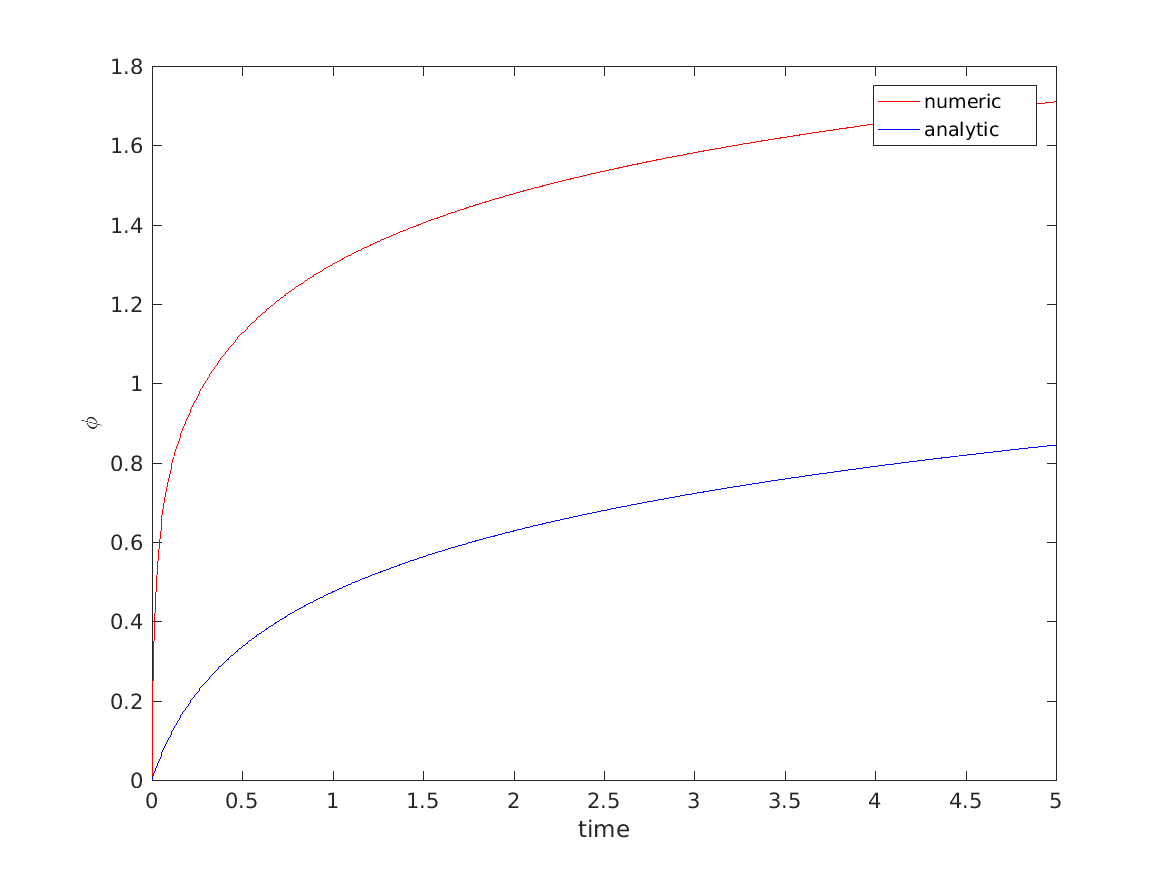
\includegraphics[width=5in]{phi_t.png}
\caption{analytic and numerical solutions of $\phi$, calculated using the exponential and exponential prefactor solutions, respectively. The parameters are set to $\lambda = 8$, $\beta$ = 34, $V_0 = 1$, $\delta = 0.005$, $\chi = 1$, $\phi_0 = \beta 1\mathrm{e}-3$. In the small $\phi$ limit, the solutions are approximately equal}
\end{figure}

\subsection{$\rho_{\phi}$ and $\rho_{\lambda}$}
lol

\subsection{Equation of state}

$w_{\phi}$ can be calculated by recalling the relations from the stress energy tensor for the field scalar field $\phi$. Namely, $w = p_{\phi} / \rho_{\phi}$, $p_{\phi} = \frac{\dot{\phi}^2}{2} - V(\phi)$ and $\rho_{\phi} =  \frac{\dot{\phi}^2}{2} + V(\phi)$. Our ODE solver gives us $\dot{\phi}$, and we know the form of the potential, so we can evaluate the equation of state for all time steps. Please see figure 3 for solution.

\begin{figure}
\centering
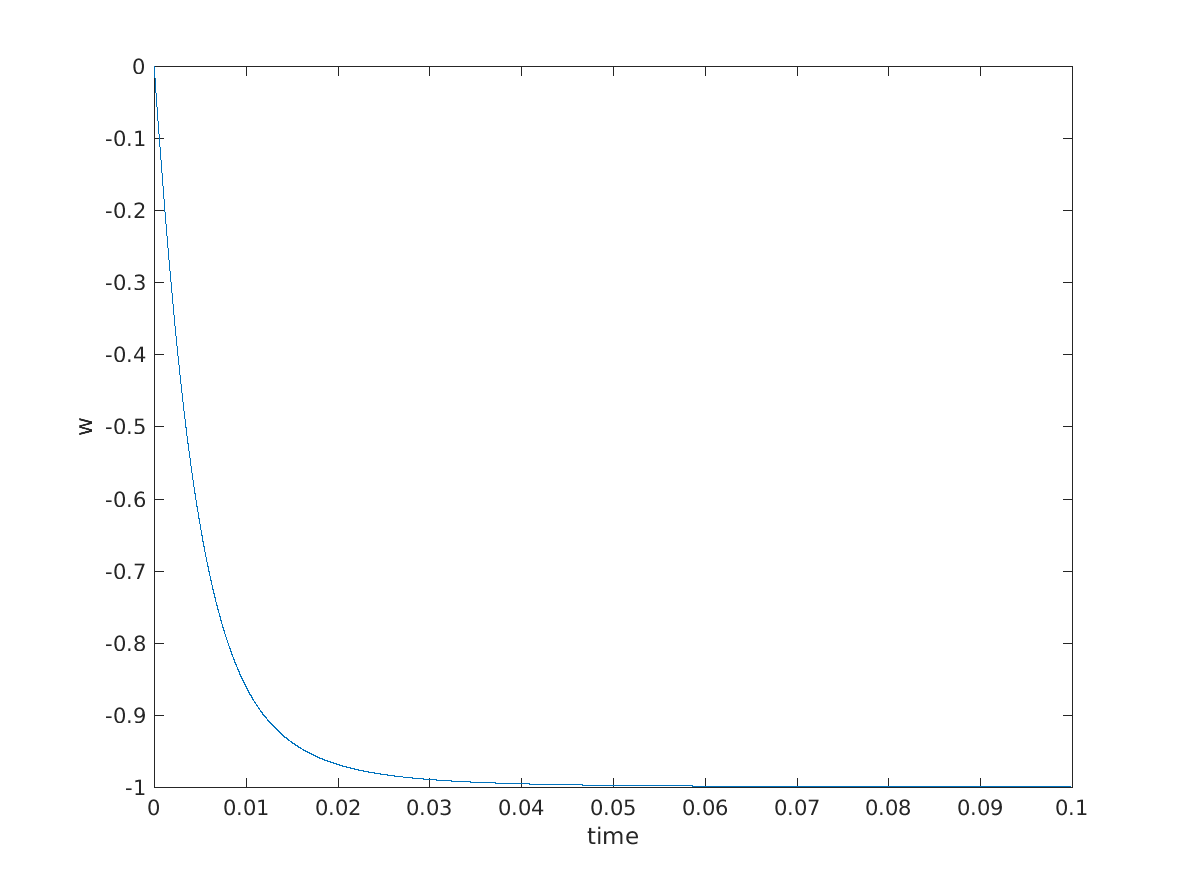
\includegraphics[width=5in]{eqofstate.png}
\caption{The equation of state for the scalar field $\phi$. We use the initial condition $\phi_{0} = 33.95$ and $\dot{\phi}$ = 2e-61. The equation of state oscillates but dampens out to -1. For such a scenario, $\dot{\phi} \to 0$ }
\end{figure}

\subsection{$\Omega_{i}$ for different scenarios}
Please see figure 4 for the solution using the results of 4.2, and figure 5 for the results of 4.3

\begin{figure}
\centering
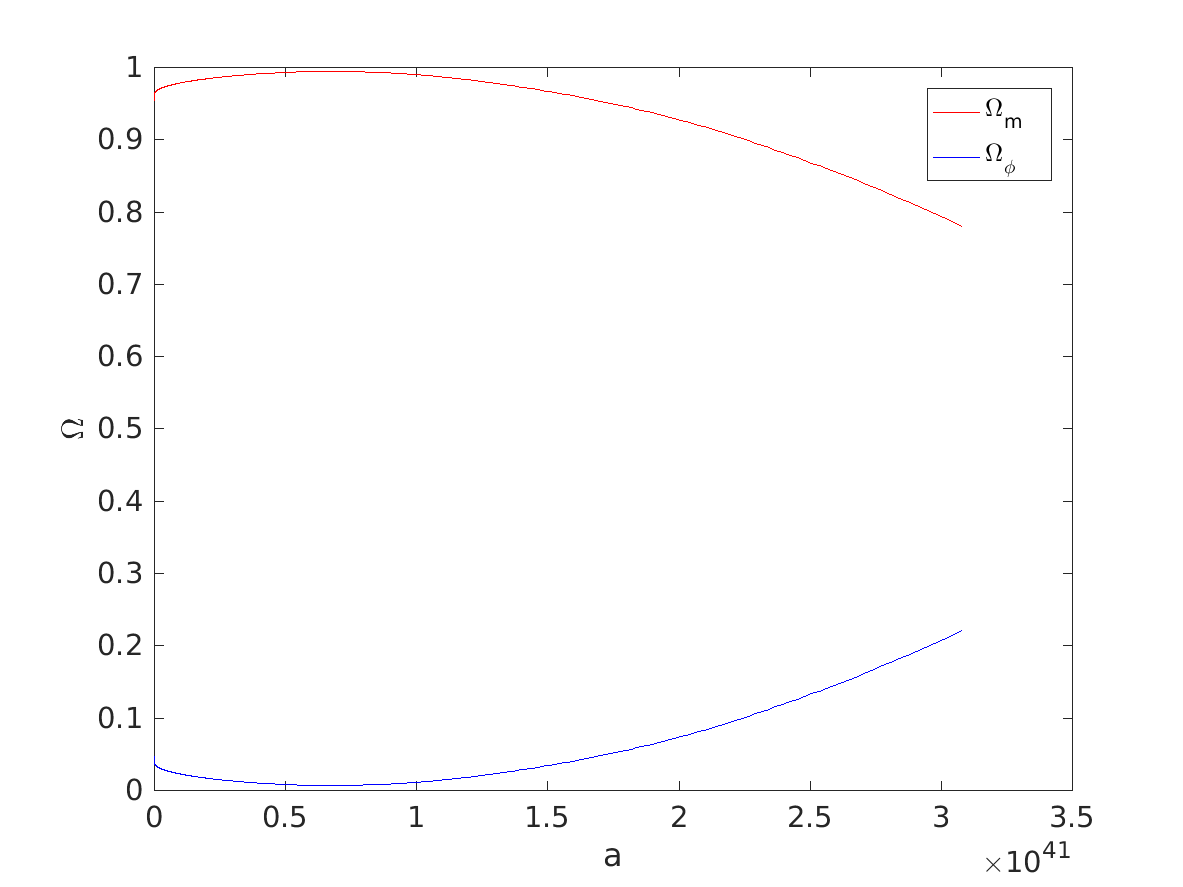
\includegraphics[width=5in]{omega_54b.png}
\caption{}
\end{figure}

\begin{figure}
\centering
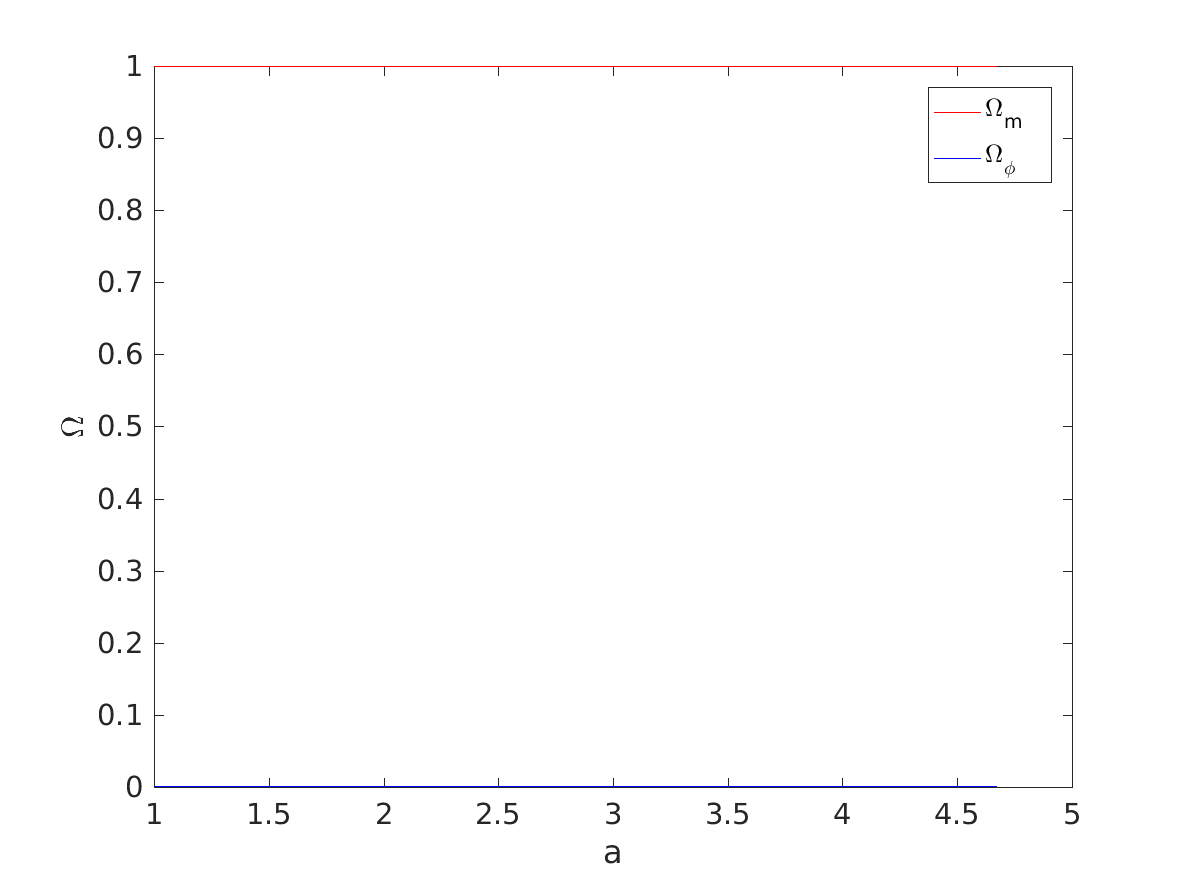
\includegraphics[width=5in]{omega_54c.png}
\caption{This universe starts out matter dominated, but as time elapses, switches over to a $\phi$ dominated universe.}
\end{figure}

\subsection{$\phi$ and $V(\phi)$ vs time}
Please see figure 6 below
\begin{figure}
\centering
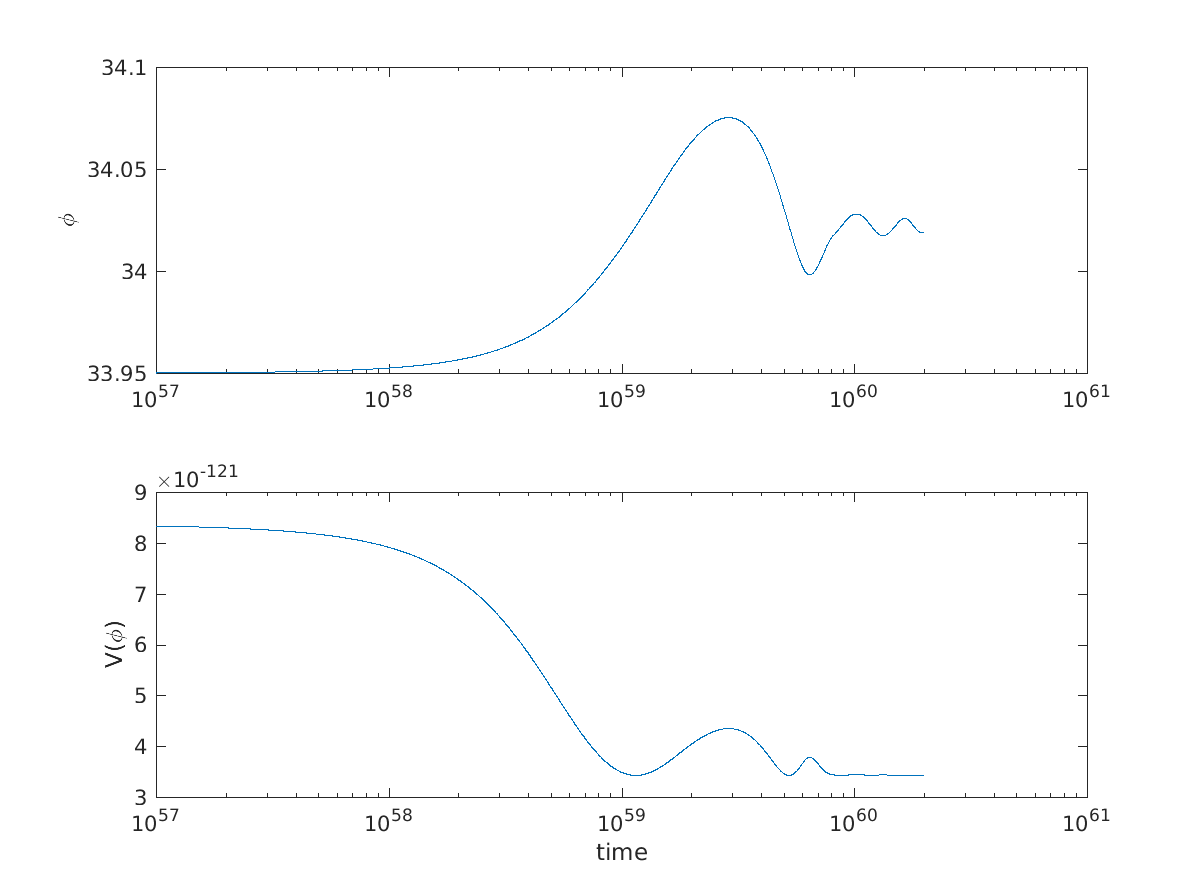
\includegraphics[width=6in]{phiVt.png}
\caption{The scalar field drops through the minima of the potential, then oscillates about it. The motion mimics that of a damped harmonic oscillator}
\end{figure}

\end{document}
